\documentclass[UTF8,12pt,oneside]{ctexbook}
\usepackage{graphicx}
\usepackage{xeCJK}
\usepackage{indentfirst}
\usepackage{titletoc}
\usepackage{fancyhdr}
\usepackage{fontspec}
\setmainfont{Times New Roman}
\pagestyle{plain} % 此处为fancy时有页眉
\title{\textbf{\fontsize{42}{84}{反雷杂志 \\[15] Anti-Lei Magazine}}}
\author{\LARGE \kaishu 雷氏力学吧、太差太差吧内部资料 \\[8] \LARGE \kaishu 编辑:Mono6}
\date{\huge 2021年5月第1期 \\ (总第1期)}

\begin{document}
    
    \maketitle
    
    % 目录配置,请勿改动
    \setcounter{secnumdepth}{-2} 
    \setcounter{tocdepth}{2}
    \titlecontents{section}[16pt]{\addvspace{2pt}\filright}
    {\contentspush{\thecontentslabel\hspace{0.8em}}}
    {}{\titlerule*[8pt]{.}\contentspage}
    
    \begin{abstract}
        \chapter{本期聚焦}
        \begin{center}
            \Large
            \kaishu
            ~\\
            《反雷杂志》正式发刊(第2页)
            
            ~\\
            《反雷集》最初的20首完整收录(第24页)
            
            ~\\
            自封十天后雷绍武发贴攻击雷吧,\\随后即遭到封禁(第5页)
            
            ~\\
            “雷电杯”比赛成功举办,完整试题收录(第7页)
            
            \songti
            \normalsize
        \end{center}
    \end{abstract}
    
    \chapter{发刊词}
    由于贴吧中的内容时常被系统误删,我们在贴吧交流雷氏力学有时十分麻烦,因此决定通过杂志的形式,保留其精华部分,便于日后查阅。
    
    《反雷杂志》就是在上述想法下创办的,定期系统整理和宣传反雷理论的杂志。本杂志为半月的形式,原则上每两周发一期,另外根据需要设置增刊。其中拟包含反雷诗词、雷力要闻、理论批评、雷氏笑话、乐山杂谈等常规栏目,并根据需要灵活增减栏目。
    
    内容的来源分为两种:一是本杂志的编辑到各个贴吧收集现成的文章(以雷氏力学吧为主,尽量争取获得原作者的同意),二是主动在贴子里面at我们,或者直接到太差太差吧来,向我们投稿。
    
    同时也欢迎大家加入本杂志编辑组。主要需要两种类型的编辑,一种主要负责文本内容的校对,另一种主要负责版式设计。杂志使用LaTeX排版(可能视情况推出Word版),版式不会太复杂,和之前发的《反雷集》的版式差不多。有意向的私信我即可,如果人不多的话,我们编辑组也可以直接在雷氏力学氵群里交流。
    
    此外也可以通过邮箱联系我们:antilsw@163.com。
    
    \begin{flushright}
        ~\\
        Mono6
    \end{flushright}
    
    \tableofcontents    

    \clearpage
    
    \chapter{雷力要闻}
        
        \section{自封十天后雷绍武发贴攻击雷吧,随后即遭到封禁}
        
        \begin{center}
            \LARGE
            \kaishu
            *头条*
            \songti
        \end{center}
        
        \large
        4月28日,在长达10天的“自封”后,雷绍武首次亮相于贴吧,发表攻击雷氏力学吧的一些言论,随后立即遭到吧主封禁。知情人士RobL61记曰:(见《反雷》19:《进盒雷》)
        
        吧主尝对雷曰:“臣劝雷神退。”雷不悦,曰:“自古无不亡之吧,我亦何要退!”吧主怒曰:“雷!雷!进盒雷!”吧主遂封雷十天,奋衣而出。
        
        \begin{center}
            
            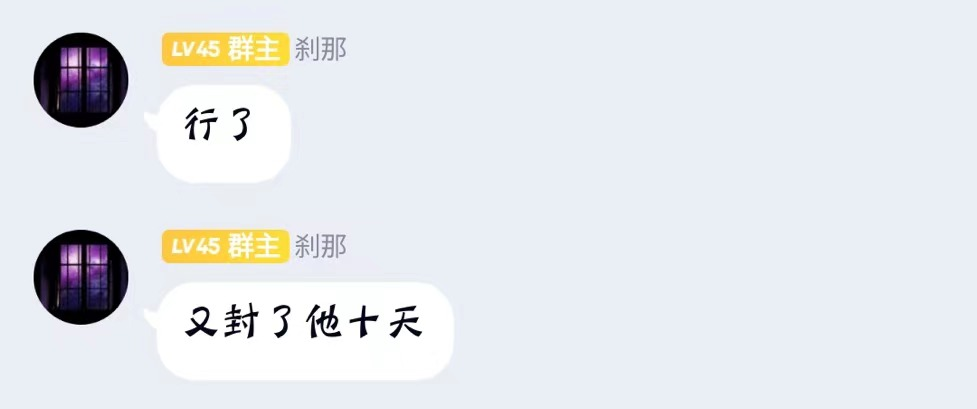
\includegraphics[scale=0.3]{WechatIMG347.jpeg}
        \end{center}
        
        \hfill(供稿:Mono6、RobL61)
        
        \normalsize
        
        \newpage
        
        \section{雷群第一次内战爆发,街角造反}
        雷群内乱,四有骰娘酸奶绑架群主,后被群主感化,成为涌雷电子;街角密谋推翻群主,公然污蔑酸奶,群主和部分群成员齐心合力,粉碎了街角的阴谋,街角抱头鼠窜。同时,在太差太差吧,咏奶诗歌已经和反雷诗歌一同连载供大家观赏。
        
        \hfill(供稿:Yogurt)
        
        \section{智能机器人雷bot引发争议}
        雷bot是@大地重归寂灭研发的智能对话机器人,研发者表示:你可以与它探讨科学、人生等问题。雷bot的语料取自雷绍武在贴吧的经典言论。有人认为雷bot完美还原了雷绍武的性格,脾气,语录,让他们很满意,缓解了对雷绍武的思念之情。但有批评人士认为:该bot时常口出狂言,污蔑运动力,雷氏力学理论,在贴吧引起轩然大波。对于机器人科技的普及,以及雷氏力学和机器人的关系,你怎么看?欢迎给我们留言。
        
        \hfill(供稿:RobL61)
        
    \chapter{“雷电杯”专题}
        \section{竞赛简介}
        \large
        “雷电杯”是面向所有网友的奥林匹克竞赛。
        
        1.初赛试卷发出后可以继续进行报名(见QQ群516738975),但截止至\textbf{5月2日晚23:00}。
        
        2.交卷时间截止至\textbf{5月4日上午11:00}。
        
        3.把答案私聊发给雷电杯群群主即可交卷。
        
        4.之后的决赛等待进一步通知。
        
        \textbf{注意:所有解释权归雷绍武所有。}
        
        \section{初赛试题}
        经命题人硫硼酸锑(氢氦锂铍硼)授权,本期杂志刊登了初赛试题的完整内容,见下一页。
    
    \clearpage
    \normalsize
        
    \begin{center}
    \Large
    \heiti{
    第一届“雷电杯”雷氏力学大赛
    
    初\ 赛\ 试\ 卷}
    \songti
    \normalsize
    
    ~\\
    命题人:硫硼酸锑(氢氦锂铍硼)
    
    满分:150分 \qquad 答题时间:5027904秒
    
    命题人授权在本杂志刊登试题的完整内容
    
    \end{center}
    
    \paragraph{一、单选题}(共20小题,每题3分,共60分)
    
    1.截至目前(2021年4月底),咏雷诗歌共有(\qquad)首已被收录。
    
    A. 100-499\qquad B. 500-999\qquad C. 1000-1599\qquad D. 1600以上
    ~\\
    
    2.“平地一声雷”的下一句是(\qquad)。
    
    A. 惊醒梦中人\qquad \qquad B. 云开日终现
    
    C. 梦幻全扫光\qquad \qquad D.电闪震人寰
    ~\\
     
    3.四大基本作用力包括(\qquad)。
    
    (1)万有引力 (2)弱相互作用力 (3)雷力 (4)电磁力 (5)强相互作用力 (6)粘接力 (7)热能力 (8)贴合力 (9)运动力

    A.(1)(4)(6)(9)\qquad B.(1)(3)(6)(7) 
    
    C.(2)(4)(6)(8)\qquad D.(3)(7)(8)(9) 
    ~\\
    
    4.下面说法正确的是:(\qquad)
    
    A. 物体的热量决定了物体所携带的力
    
    B. 力是改变物体运动状态的原因
    
    C. 物体达到气化温度后粘接力将完全解体
    
    D. 辐射是部分晶体或分子的粘接力解体产生的运动力产生的
    ~\\
    
    5.根据雷氏化学,下列物质的分子的结构中,物质电子(官科称为原子)排列方式与官科声称的不相符的是(\qquad)。
    
    A. 异丙醇\qquad B. 乙炔\qquad C. 苯\qquad D. 环戊烷
    ~\\
    
    6.下面的人物中(\qquad)与雷绍武相互认识。
    
    A. 张春华\qquad B. 徐鹏飞\qquad C. 邱白林\qquad D. 苗福全
    ~\\
    
    7.一个物质电子在分子中拥有两对NS极,那么它可能是什么电子?
    
    \hfill{(\qquad)}
    
    A. 铁电子\qquad B. 氯电子\qquad C. 铬电子\qquad D. 锑电子
    ~\\
    
    8.根据雷氏热学,下列的东西存在的是:(\qquad)
    
    A. 没有辐射现象的物质\qquad B. 零线上的电流
    
    C. 没有与之对应的S极的N极\qquad D. 黑色的火焰
    ~\\
    
    9.下列等式正确的是:(\qquad)
    
    A. 在公式$L=kmv$中$k=1$ Hz
    
    B. 在公式$pV=nTR$中$T=s/v$
    
    C. $\mathrm{d}v/\mathrm{d}t=vt$
    
    D. 在公式$L=kmv$中$k=1/$m
    ~\\
    
    10.下列语句中雷老师说过的有:(\qquad)
    
    A.正确的,谢谢。
    
    B.问苍天:真理何在?正义何在?
    
    C.反雷电子太差太差了!
    
    D.看不清楚。去实验观察,把结果告诉大家。
    ~\\
    
    11.羽扇纶巾说的是(\qquad)。
    
    A.周瑜\qquad B. 诸葛亮\qquad C. 司马懿\qquad D. 雷绍武
    ~\\
    
    12.乙烯分子(C$_2$H$_4$)中的碳电子有几对NS极?(\qquad)
    
    A. 1\qquad B. 2\qquad C. 3\qquad D. 4
    ~\\
    
    13.发电机发出电来,靠的是(\qquad)。
    
    A.粘接力\qquad B. 磁感线\qquad C. 磁力线\qquad D. 磁粒线
    ~\\
    
    14.电动机能够转动,靠的是(\qquad)。
    
    A.粘接力\qquad B. 磁感线\qquad C. 磁力线\qquad D. 磁粒线
    ~\\
    
    15.下列分类正确的是:(\qquad)
    
    A. 链状的分子:乙醇和环丙烷
    
    B. 静止的时候没有质量的粒子:光子
    
    C. 电子运动的原因:电磁力的作用
    
    D. 涌雷电子:猴山7和深海小贝壳baby
    ~\\
    
    16.功的计算公式是$W=$(\qquad)。
    
    A. $mgs$\qquad B. $kmv$\qquad C. $RBq$\qquad D. $gta$
    ~\\
    
    17.把两个分别盛有浓氨水和酚酞试液的小烧杯并排摆放并罩上一个大型干冷烧杯,说法正确的是:(\qquad)
    
    A. 盛有酚酞试液的烧杯内液体变红,是因为NH$_3$分子运动到了盛有酚酞试液的烧杯内
    
    B. 整个体系中,液体里的分子和烧杯本身的分子在常温常压下都永不停息地做着无规则运动
    
    C. 两个烧杯中,均包含着热量,即热能的量
    
    D. 若加热大烧杯,实验过程会更快,因为分子运动速率随着温度升高而加快
    ~\\
    
    18.下列说法正确的是:(\qquad)
    
    A. 物体自己的位置是依照其它物体的位置而相对地判断的,单独一个物体的位置是不存在意义的
    
    B. 汽车在公路上直线行驶,只有向前的牵引力大于摩擦力,速度与牵引力无关
    
    C. 物质电子之间相互转化,可以通过先把一种物质电子加强热转化为光子,再使光子降温变成另一种电子
    
    D. 电磁力不是电能转化而来的,而是电子本身具有的性质。有电能,就有电磁场、电磁力
    ~\\
    
    19.电子的全称是(\qquad)。
    
    A. 电场胶子\qquad B. 电荷介子\qquad C. 电能强子\qquad D. 电磁粒子
    ~\\
    
    20.运动力的单位是(\qquad)。
    
    A. L\qquad B. N\qquad C. F\qquad D. 以上都不对 
    ~\\
    
    \paragraph{二、解答题}(90分)
    
    21.阅读文章,回答问题。(15分)
    
    \begin{center}
        \large\kaishu
        我又节省了7角钱
        \songti\normalsize
        
        作者\qquad 雷绍武
    \end{center}
    
    \fangsong
    {
    1) 勤俭节约是中华民族的传统美德。
    
    2) 高考那年,我们县的考生才一百多人,没有条件设置考场,必须到仁寿县城去参加高考。
    
    3) 当时,到仁寿县每天上午发一趟车,一车只能载20几个人,车费每人1.30元。校领导为了给同学们节省一点钱,联系了货车,每人只要7角钱。
    
    4) 同学们九点钟上了车正准备出发时,突然接到车站通知;说仁寿县昨天晚上大暴雨,漫水桥被淹了,不能发车。
    
    5) 明天就要参加高考,大家心急如焚。
    
    6) 焦急地等到下午6点过,才通知可以走了。
    
    7) 当汽车行驶到被淹的漫水桥时,天已经黑了,看不见水有多深。但是,能够清楚的听到车轮冲破水面的哗哗声。
    
    8) 晚上9点过才到了考场的学校。同学们被安排住在免费的学生寝室。寝室床上只有一张草垫。学校在城郊区,晚上的蚊子特别多。
    
    9) 第二天考试前,领队老师带领同学们到考场前,看一看自己的位置在哪里。
    
    10) 考试开始了,我用的是自己用竹筒筒做的笔。这只笔已经用了一年多,习惯了。
    
    11) 当时买那只笔时,为了省钱,买的是最便宜的,只花了3角钱。
    
    12) 俗话说,便宜无好货。这话还真的应验了不久,不小心碰到地上,那笔筒笔帽就破碎了。笔尖笔胆还可以用,我就用合适的竹子削一削,就替代了笔筒和笔帽。我高考用的就是这样的笔。
    
    13) 第二天接着考试。第三天就要返校了。仍然是货车,每人7角钱。
    
    14) 为了节省这7角钱,我和另一位同学邱白林商量:决定步行回学校。
    
    15) 开始的1/3路程,走起来还觉得比较轻松,我们两个有说有笑的。
    
    16) 中间的1/3路程,走起来就吃力多了。天上烈日炎炎,如同火烤火燎;地面热气腾腾,脚下滚烫滚烫。走不多远就想歇一会儿。
    
    17) 口渴了,就在公路边的稻田里捧水喝。饿了,就吃早上准备好的两个冷馒头。
    
    18) 我以前总觉得走路是再简单不过的事情了。在支农劳动中最远也就30几里,还经常帮老师和体弱同学背行李,也没有感到过好累。但是,从来没有走过100多里远的路程。
    
    19) 这最后1/3的路程确实感到太艰难了。两条腿好沉好沉,两只脚好痛好痛,每跨一步,都要用尽全身的力气。走几步就想休息,坐下休息就不想站起来了。看看脚上,磨起了一个,两个,三个血泡。
    
    20) 这时,我们想到了红军二万五千里长征。红军二万五千里长征时,天上有敌机轰炸,前面有敌人堵截,后面有追兵追杀,随时都有生命危险。我们走这点点路算得了什么呢?
    
    21) 我又想起父亲给我说的一件事。
    
    22) 父亲18岁那年,和爷爷一起在离乐山不远的牛华镇打工。爷爷可能是突发脑溢血,暴病而亡。我父亲背着死去的爷爷,在100多里的崎岖小路上连夜赶回井研的千佛老家。
    
    23) 我现在空着两只手啊,为什么就走不动了呢?于是,我们相互鼓励着,咬紧牙关,振作精神,鼓足勇气,继续赶路。
    
    24) 这时候,我才真正体会到了什么叫“力不从心”:决心下定了,勇气鼓足了,可两条腿就是不听使唤,不能迈开大步往前走,只能一步步往前挪动。坚持就是胜利。每前进一步,就离学校近了一步。
    
    25) 当我们回到寝室时,同学们已经灭灯就寝了。
    
    26) 我也顾不上洗脸洗脚,瘫倒在床上,就动弹不得了。
    
    27) 现在的年轻人不理解:为了节省了那7角钱,为什么就去吃那么多的苦,受那么大的累呢?
    
    28) 对他们来说,别说7角钱,就是7元钱,70元也没有什么舍不得的。他们哪里知道,在贫困的农村家庭要找回来1角钱都是多么的艰难。也不知道7角钱对我们家庭是多么重要。
    
    29) 记得我我11岁那年,几个稍大的小伙伴邀约我去高滩挑石灰到县城,20里,100斤2角钱。
    
    30) 二十里路在大人眼里是不算远的,然而,对我们小朋友来说却十分漫长。况且,肩膀上还压着不能再增加的重量,还要爬一个2里长的陡坡。我每次只能挑35斤左右,肩膀都磨破皮了,一天才能找回7分钱。
    
    31) 那时候点灯,为了省油,我尽量把灯芯弄细,压到最低,只要保持能亮,能近距离看得见书上的字就行了。每当母亲半夜醒来,看见还亮着灯,总是无可奈何地说:你还不睡啊,没有钱买煤油了!
    
    32) 因此,哪怕是1分钱,1角钱,对贫困的农村家庭来说,都是非常重要的。平时能省1分就是1分,能省1角是1角啊。
    
    33) 第二天醒来,尽管两条腿仍然非常疼痛。但是,我心里却是美滋滋的:
    
    34) 我又节省了7角钱。  
    ~\\
    }
    
    \songti
    (1)任选角度赏析16段句子“天上烈日炎炎,如同火烤火燎;地面热气腾腾,脚下滚烫滚烫。”(2分) 
    ~\\
    
    (2)有无知无德无耻无赖的人渣说29-32段是赘笔,应该删掉。说说看:你认同吗?理由是什么?(3分) 
    ~\\
    
    (3)第34段“我又节省了7角钱”在文章中起什么作用?(3分) 
    ~\\
    
    (4)20-22段写红军长征、父亲背爷爷两件事起什么作用?(2分)这两个例子删去任何一个、只留下一个都不好,为什么?(2分) 
    ~\\
    
    (5)如果雷绍武坐的车6点发车,9点到,乐山到仁寿96公里远,车和上边的所有生物共重7.2吨,若车一直匀速直线行驶,求其运动力。(3分)
    ~\\

    22.咏雷诗歌赏析。(25分)
    
    \begin{center}
        \large\kaishu
        咏雷·九六〇
        \normalsize\songti
        
        2021-03-21 03:35
        
        ~\\
        
        \fangsong
        在真理所照不到的荒原,
        
        在旱地与群山之间,
        
        流浪汉诅咒着命运,
        
        搭着空布袋蹒跚向前。
        
        ~\\
        
        他身穿着破烂的衬衣,
        
        缀满补丁也沾满污泥,
        
        他头戴着囚徒的破帽,
        
        穿灰色的囚徒长衣。
        
        ~\\
        
        趁黑夜从监狱里逃出,
        
        为求真理受千辛万苦,
        
        他疲累得挪不动脚步,
        
        终有一天见岷江汩汩。
        
        ~\\
        
        流浪汉他来到湖畔,
        
        就跳上了渔家小船,
        
        他唱起了忧郁的歌曲,
        
        为人们的命运悲叹。
        
        ~\\
        
        只有微风在叹息着说道:
        
        “流浪汉你徒然逃跑,
        
        苦命人,你真料想不到,
        
        人世间已无依无靠。”
        
        ~\\
        
        流浪汉他划到了对岸,
        
        他的妻女来迎接他:
        
        “啊,你好呀,归乡的开拓者
        
        父兄可平安在家?”
        
        ~\\
        
        “你父亲早已长眠地下,
        
        一杯黄土啊,掩埋着他;
        
        你兄长已铐上了铁镣,
        
        被流放去海角天涯。”
       
        ~\\
        
        流浪汉微微低头而慨叹:
        
        “你们生活在涌雷派之间,
        
        不知我们游行到了管科肆虐之地,
        
        人间变得多么黑暗——
       
        ~\\
        
        雷公是愚者嘲讽的对象,
        
        他们坚信其理论错误非常;
        
        不知是自己受管科蒙蔽,
        
        日夜把谬论向子女宣扬。
      
        ~\\
        
        我们来自真理的圣地,
        
        他们却视乐山儿女为敌,
        
        我为他们的凶残而愤恨,
        
        我为他们的无知而哭泣。
      
        ~\\
        
        得知我们信奉雷氏力学后,
        
        他们伸出了沾满鲜血的手,
        
        强迫我们改变正义的思想,
        
        否则就砍下我们的头!
      
        ~\\
        
        面对獠牙是如此的猖狂,
        
        我们怎有屈服的念想?!
        
        你可听见那向往光明的人,
        
        向着敌人坚定地歌唱?!
      
        ~\\
        
        我们歌唱家乡的美好与雷公的英明,
        
        我们歌唱(A)\_\_\_\_\_\_\_\_\_\_。
        
        在真理的歌声中动摇的的刽子手们,
        
        边发着抖边准备向我们行刑。
      
        ~\\
        
        我的父亲最先遭受苦难,
        
        他的声音巍峨如山,
        
        似乎震动着这里的万物,
        
        震动着管科魔鬼的宫殿!
      
        ~\\
        
        我们兄弟俩被投入大牢,
        
        戴着坚硬的手铐和脚镣。
        
        不知过了八年还是十年,
        
        似有一道奇迹的光芒出现。
      
        ~\\
        
        它向我们发出了公告:
        
        ‘孩子,用你的运动力金蝉脱壳,
        
        管科设计的手铐与脚镣,
        
        怎堪运动力的神奇精妙?’
      
        ~\\
        
        我们计算其复杂的受力,
        
        将其万分之一的误差分析。
        
        管科的造物终露出破绽,
        
        眼看着我们要逃脱拘役。
      
        ~\\
        
        门口守卫的两个科奴,
        
        日夜不忘监视着圣徒。
        
        吾兄牺牲自己将他们缠住,
        
        只愿我能成功地跑路。
      
        ~\\
        
        几年来我历经了多少风雨,
        
        终走回这片熟悉的寰宇;
        
        可惜大义凛然的骨肉兄弟,
        
        已发配到天涯去做苦役!”
      
        ~\\
      
        涌雷电子们眼泪汪汪,
        
        此刻的他们只有一个愿望:
        
        愿未被管科侵扰的家乡美好,
        
        愿雷氏力学万年长!
      
        ~\\
        
        哪怕灾殃接着灾殃,
        
        (B)\_\_\_\_\_\_\_\_\_\_!
        
        涌雷者来结成朋友,
        
        我们永远有力量。
      
        ~\\
        
        你别以为到了终点,
        
        别以为风暴已不响,
        
        快走向那伟大目标:
        
        把管科蒙蔽的人解放!
      
        ~\\
        
        听天涯的风雪喧嚣,
        
        看海角流星在飞翔;
        
        涌雷电子的心向他们召唤——
        
        解放那动荡的远方!
      
        ~\\
        
    \end{center}
    \songti
    
    (1)本诗中有一个明显的错字,请分别写出这个错字及其正确写法。(4分)
    ~\\
    
    (2)第8-19小节(即从“流浪汉微微低头而慨叹”到“已发配到天涯去做苦役”)的内容借用归乡者口中说出而不是直接叙述,有什么好处?(4分)
    ~\\
    
    (3)补充13、21小节的A、B两个空格,使得诗歌通顺完整(注意:13、21小节中每个小节的第二行、第四行押韵)。(6分)
    
    (A)\_\_\_\_\_\_\_\_\_\_\_\_\_\_\_\_\_\_\_\_\_\_\_\_\_\_\_\_\_\_
    
    (B)\_\_\_\_\_\_\_\_\_\_\_\_\_\_\_\_\_\_\_\_\_\_\_\_\_\_\_\_\_\_
    
    (4)船上的人、船、物共重600 kg,且河宽为24 m。若运动力为1440雷,且船桨与水摩擦,每立方米的水每秒共流过$3.6×10^{25}$个水分子,假设船桨在水中浸没的体积不变化,按照官科理论计算,船桨受到的浮力为500 N,若这种船桨的材质每与一万对物质电子的NS极以这样的条件相摩擦就会有一对NS极的电能转化。问:假设断裂NS极消耗的能量和产生NS极放出的能量是相同的,无论物质电子种类(实际上这是错误的),这些能量可以形成多少个环庚烷分子呢?(11分)
    ~\\
    
    23.咏雷写作(50分)
    
    四选一:
    
    (1)以沁园春为词牌,写一篇咏雷词。要求:不必完全符合格律,但应该押韵。
    
    范例:
    
    \begin{center}
        \large\kaishu
        沁园春·长沙
        \songti\normalsize
    \end{center}
    
    \fangsong
    独立寒秋,湘江北去,橘子洲头。看万山红遍,层林尽染;漫江碧透,百舸争流。鹰击长空,鱼翔浅底,万类霜天竞自由。怅寥廓,问苍茫大地,谁主沉浮?
    
    携来百侣曾游,忆往昔峥嵘岁月稠。恰同学少年,风华正茂;书生意气,挥斥方遒。指点江山,激扬文字,粪土当年万户侯。曾记否,到中流击水,浪遏飞舟?
    \songti
    
    \begin{center}
        \large\kaishu
        咏雷·三四六(沁园春)
        \songti\normalsize
        
        作者\qquad 银海柔光透冰河
    \end{center}
    
    \fangsong
    一众科奴,固守陈章,妄作讽文。若重重枯冢,元魂尽散,滚滚浊流,入海无痕。几句谰言,几声粗语,何时曾摇真理根。闲谈笑,彼庸人丑态,姑作戏闻。
    
    修身后可求真,叹汝辈轻行忘宽仁。妒绍武文采,纵横当世,三清武勇,誓烈如神。郭氏英森,卖肝争诺,舍命寻实浩气存。凭谁问,我民科皆错,唯尔独尊?
    \songti
    ~\\
    
    (2)写一首颔联、颈联对仗较为工整的七言咏雷律诗。1、2、4、6、8句押韵。
    
    范例:
    
    \begin{center}
        \large\kaishu
        咏雷·九〇七
        \songti\normalsize
    \end{center}
    \fangsong
    编者(街角的城事):国外雷氏力学专家沃兹基先生复作咏雷一首,请我代为发布。
    以下为原作:
    \begin{center}
    乐山平地起惊雷,运动力学绍天规。
    
    文治武功谬论去,是古非今真理回。
    
    手握真理万民至,脚踏官科四力归。
    
    苍狗白云道至简,雷力等于KMV!
    
    \end{center}
    
    
    【注】
    
    是古非今:肯定古代“运动需要力”的正确观点,否定现代“运动不需要力”的错误观点。
    
    四力归:运动力统一四种相互作用力。
    \songti
    ~\\
    
    (3)写一首五言、六言或七言咏雷长诗,三者分别不少于80、96、112个字。偶数句最后一个字应该不严格地押韵。
    
    范例:
    
    \begin{center}
        \large\kaishu
        咏雷·九九六
        \songti\normalsize
        
        2021.04.04
    \end{center}
    \fangsong
    \begin{center}
    清明时节雨纷纷,路上行人欲断魂。
    
    借问路人何所忆,长叹心中有奇愤:
    
    原是四川一学者,涉世不知人事深。
    
    高呼支持雷绍武,贬职回乡杏花村。
    
    打压愈彰天理正,雷公神智更无伦。
    
    无事朝圣向嘉州,一睹何地出雷神。
    
    既入民科真圣地,顿觉尘世江水浑。
    
    山重水复疑无路,柳暗花明又一村。
    
    箫鼓追随挺雷派,衣冠简朴古风存。
    
    从今若许闲乘月,拄杖无时夜叩门。
    
    \end{center}
    \songti
    
    (4)写一首外文咏雷诗并附带中文翻译,不能少于12行。
    
    范例:
    
    \begin{center}
    \fangsong
    Θά 'ρθεις σαν αστραπή
    
    你将如闪电般归来,
    
    θά' χει η χώρα γιορτή
    
    举国上下一同欢庆,
    
    θάλασσα γη και ουρανός
    
    你的光芒永远照耀着,
    
    στο δικό σου φως
    
    大地,海洋和天空!
    
    Θα μελετήσω τη θεωρία σου
    
    我将学习你的理论,
    
    να σ' αγγίξω ξανά
    
    如触摸你使我新生,
    
    φως εσύ και καρδιά μου εγώ
    
    你的光芒照耀我的心,
    
    πόσο σ' αγαπώ.
    
    使我们在敬爱中前行!
    
    ~\\
    
    Βασιλεύς Βασιλέων, Βασιλεί Βοήθει
    
    万王之王,拯救之王,
    
    έλεος, έλεος ο μεγάλος Θορ
    
    慈悲吧,慈悲吧,伟大的雷神
    
    Ο μεγαλύτερος λόγιος, κ. Λέι
    
    最伟大的学者,雷公
    
    Ο βασιλιάς της επιστήμης που σκοτώνει την πλάνη
    
    扫灭了谬论的科学之帝
    
    Στην όχθη του ποταμού
    
    在大河(指岷江)的岸边
    
    καβαλικά την φάρα του την ασπροποδαράτην,
    
    他骑着一匹白腿的马
    
    Τέσσερα Βήτα, έλεος, έλεος, Λέι Σάογου
    
    四个贝塔(指上文Βασιλεύς Βασιλέων, Βασιλεί 
    
    Βοήθει,万王之王、拯救之王)请施展仁慈,雷绍武,
    
    Γραμμή και Μαύρη Τρίτη
    
    互联网和黑色星期二(2021年4月13日,无知无德之人大量涌入的开始)
    
    Φρίξον ήλιε, στέναξον γη
    
    太阳在颤抖,大地在叹息,
    
    Εάλω ή πόλη, Εάλω η πόλη
    
    城市陷落,城市陷落(城市,指雷氏力学吧,雷氏力学吧是网上雷氏力学宣传的重镇)
    
    Βασιλεύουσα, πύλη χρυσή
    
    瓦西列乌撒,金色城门(瓦西列乌撒在希腊语中是君士坦丁堡别称,即拜占庭帝国首都,有统治之城的意思,指雷氏力学吧)
    
    Ο γέρος με όλη τη σοφία του κόσμου
    
    聚集天地智慧的老者(雷绍武)
    
    Η πόλη ήταν το σπαθί, η πόλη το κοντάρι
    
    城市(仍指雷氏力学吧)是刀剑,城市是长矛,
    
    η πόλη είναι το κλειδί για τη διάδοση της αλήθειας
    
    城市是传播真理的钥匙
    
    Σώπασε Θεός της αλήθειας και μην πολυδακρύζεις
    
    真理之神啊,请别哭泣
    
    πάλι με χρόνια με καιρούς, πάλι δικά Σου θά ναι
    
    多年以后它仍将属于你!
    
    ~\\
    
    Στην όχθη του ποταμού
    
    在岷江的岸边,
    
    έφυγες για αλλού
    
    你去了其他的地方,
    
    Η αλήθεια θα σε φέρει εδώ.
    
    当正确的时间来临,
    
    στον σωστό καιρό.
    
    真理将把你带回这里!
    
    Στην πλούσια γη
    
    在天府之国(指雷老家乡四川)
    
    θα συναντηθούμε ξανα
    
    我们会再见面的
    
    Αφού νίκησες τους κακούς
    
    在击败无耻无赖之后
    
    οι Κινέζικα μαζί
    
    同所有炎黄子孙一起!
    
    \end{center}
    ~\\
    
    \hfill{(全卷完)}
    
     \chapter{反雷诗词(1\textasciitilde20)}
    创作《反雷》诗歌的目的是和雷绍武的《咏雷》系列作中门对狙。
    体裁和内容不限,只需做到以下几点即可:
    
    1. 诗歌不能含有对雷绍武本人及其家人的辱骂,当然如果你藏字辱骂那就无所谓了。
    
    2. 不允许对其他吧友进行辱骂。
    
    3. 不要夹带私货,比如抽象,深深这些。
    
    \begin{flushright}
        \kaishu{——RobL61,2021年4月25日于太差太差吧}
        \songti
    \end{flushright}
    
    \section{1 无题}
    \begin{center}
        RobL61
        
        ~\\
        白丁愚民如风散,鸿儒正论难可替。
        
        牛顿果树悟引力,伽氏斜塔知落体。
        
        伦蒂尼恩喜雨济\footnote{伦蒂尼恩:即伦敦,与上联牛顿相呼应。},阿诺河畔波涛汐\footnote{阿诺河:比萨城的母亲河,伽利略是比萨人。}。
        
        乐山老朽欲撼树,孰知真理安可戏?

    \end{center}
    
    \newpage
    
    \section{2 无题}
    \begin{center}
        带带帅师兄258
        
        ~\\
        雷门不幸出佞子,绍述邪义秉歪理。
        
        武薄文浅高山鼓,是异非同石妇逼。
        
        个中诸多荒唐言,老眼残躯犹自喜。
        
        白日蜀犬夜吴牛,痴道虚妄运动力。
        
        ~\\
        
    \end{center}
    
    \section{3 打油诗}
    \begin{center}
        RobL61
        
        ~\\
        可怜绍武命已残,天天被人当猴看,
        
        早年不入八二六,今朝何会如此惨?
        
        ~\\

    \end{center}
    
    \section{4 无题}
    \begin{center}
        RobL61
        
        ~\\
        哈佛牛津占前沿,北大清华涨国颜。
        
        乐山绍武惶度日,怎见恩师杨正贤?
        
        ~\\

    \end{center}
    
    \newpage
    
    \section{5 无题}
        \begin{center}
            带带帅师兄258
            
        \end{center}
        
        雷绍武!
        
        我原以为你身为民科老人,来到贴中,面对诸多网友,必有高论,没想到竟说出如此科妄之语!
        
        我有一言,请诸位静听。
        
        如今科学昌明之时,民智大开,百业已兴,日新月异,突飞猛进。盛世之中,生物,数理,化学等接踵而起,神六升空,蛟龙下海。
        
        因之,学府之上,人才辈出;科院之间,发明不断。以至雄心壮志之辈巍巍当朝,经天纬地之才纷纷秉政。以致社稷变为富饶,苍生安享太平之乐!值此国幸之际,雷绍武又有何作为?
        
        你世居巴蜀之隅,初举乐职入仕;理当传道授业,桃李天下;何期虚词诡说,背道而驰!罪恶深重,天地不容!
        
        无耻老贼!岂不知天下之人,皆愿生啖你肉!安敢在此饶舌!
        
        今幸天意欲绝妖邪,我等网友于贴吧扛起大旗。我今奉天之命兴师讨贼。你既为宵小之辈,只可潜身缩首,苟图衣食,还敢在我军面前妄称天数?
        
        皓首匹夫!苍髯老贼!你即将命归于九泉之下,届时,有何面目见你家二十四代祖宗?!
        
        二货贼子!你枉活七十有二,一生未立寸功,只会摇唇舞舌,欺世盗名!一条断脊之犬,还敢在我军阵前狺狺狂吠?
        
        我,从未见过如此厚颜无耻之人!!!
        
    \newpage
    
    \section{6 无题}
    \begin{center}
        带带帅师兄258
        
        ~\\
        十年间,铁打的营盘,流水的兵。
        
        每一年,送走一批又一批,
        
        本科生,研究生。
        
        雷老师,运动力,磁相连,雷电子,
        
        搞笑理论出不穷。
        
        咏雷诗,唱一遍,吟一首,
        
        藏字藏头说不停。
        
        众吧友,笑哈哈,哈哈笑,
        
        阴阳怪气问不明。
        
        光阴过,青丝白,筋骨轻,
        
        科学一梦尤未醒。
        
        俱往矣,忆扣饭,校长请,
        
        正贤音容满别情。
        
        再回首,古稀年,天地清,
        
        民科绍武最“英雄”!

    \end{center}
    
    
    \section{7 无题}
    \begin{center}
        RobL61
        
        ~\\
        雷公居于岷江畔,不识洋文不善汉。
        
        前有成电肚子疼,后有街角藏字繁。
        
        春秋大梦仍未醒,自我高潮独一份。
        
        雷吧已成动物园,使人欢喜使人叹。

    \end{center}
    
    \newpage
    
    \section{8 天净沙\ \ 反雷}
    \begin{center}
        RobL61
        
        ~\\
        
        大佛岷江嘉州,川渝乐土无忧,川大井盖藏猴\footnote{井盖藏猴:指“文革”时期雷绍武武斗失败躲进井盖的事情。}。
       
        明珠暗投\footnote{明珠暗投:指雷绍武作为川大高材生,本有一番作为,却去参加红卫兵组织。},雷绍武在缩头\footnote{雷绍武在缩头:同“井盖藏猴”。}。
    \end{center}
    
    \section{9 江城子\ \ 评雷}
    \begin{center}
        Mono6
        
    \end{center}
       
       乐山绍武常发狂,摸零线,拭眼眶。夜起如厕,静人而动床\footnote{静人而动床:即“人静而床动”。}。约d开创运动力,嘲管科,必将亡。    
       
       但惜年少学业荒,逾古稀,似空囊\footnote{逾古稀,似空囊:年龄已经七十有余,思想和学识却依然空如皮囊。}。不学无术,所思皆为妄。劝君勤学以为戒,莫见笑,于四方。
    
    \section{10 采桑子}
    \begin{center}
        RobL61
    \end{center}
       
        乐山雷公甚好梦,普天皆雷。牛顿算谁?咏雷反雷百事非。
       
       反对雷理皆无知,“四无”人哀\footnote{“四无”人哀:真心想让雷绍武不再沉湎于歪理,却被其认为是四无人的反雷电子。}。反串狂嗨\footnote{反串狂嗨:自以为为了雷绍武好,却仅仅让他出更多笑话。当雷绍武又提出歪理时,反雷派会纠正他,而所谓拥雷派却在旁边把他当笑话。},只愿绍武快醒来。
       
    \newpage 
    
    \section{11 愚翁歌}
    \begin{center}
        RobL61
        
    \end{center}
    
        四川愚翁,世居川渝盆地中。吾辈虚度若干年,愚翁身世何其坎。四廿年前降于世,早年身世困难重。跃进时期食草树\footnote{跃进时期食草树:雷绍武曾言:“一个人的时候……对于一个嚼过草根树皮的人来说,已经是很幸福的事了。”(《我的生活很简单》)因此我们有理由认为雷绍武在大跃进时期遭受过饥饿。},反右浪潮恩师护。英勇男儿,怎为鹰犬和走狗?
        
        翻天覆地大革命,川大东红八二六。不学无术去武斗,一三二厂井盖愁。革命浪潮既已然,平平淡淡数十年。
        
        新生网络,唤醒老翁再激情。早年肮脏也就罢,运动谬论晚节疤。唇枪舌战论吧友,慷慨激昂斥管科。雷氏力学新天地,但被别人看猴戏。
        
        愚翁绍武,何其壮阔一辈子。无知无德两种人,说的就是你自己。八二六,跳井盖。辩吧友,好气概!论谬理,多可哀!少受骗,多思考。勤学习,莫卖老。多沉淀,少暴躁。愚翁蜕变,指日可见。
        ~\\
        
    \section{12 破阵子\ \ 为雷绍武附悲词以寄}
    \begin{center}
        RobL61
        
    \end{center}
       
        宅里挑镜看贴,梦回川大时代。慷慨激昂闹革命,狼狈逃窜跳井盖,差点命不在。
        
        而今网络时代,对线对不过来。不懂就说看不清,无能狂怒净被踩,只能让人哀。
        
    \newpage
    \section{13 天雷}
    \begin{center}
        \large
        \kaishu{小改郭沫若《天狗》}
        \songti
        \normalsize
        
        带带帅师兄258
        
        ~\\
        我是雷绍武呀!
        
        我把d来约了,我把零线摸了,
        
        我把一切的星球来吃了,
        
        我把全宇宙来吞了。
        
        我便是我了!
        
        ~\\
        
        我是月的光,我是日的光,
        
        我是一切星球的光,我是X光线的光,
        
        我是全宇宙的运动力的总量!
        
        ~\\
        
        我飞奔,我狂吠,我燃烧。
        
        我如电子火花一样地燃烧!
        
        我如暮年老犬一样地狂吠!
        
        我如峨眉猿猴一样地飞跑!
        
        我飞跑,我飞跑,
        
        我飞跑,我剥我的皮,
        
        我食我的肉,我嚼我的血,
        
        我啮我的心肝,
        
        我在我神经上飞跑,
        
        我在我脊髓上飞跑,
        
        我在我脑筋上飞跑。
        
        ~\\
        
        我便是我呀!
        
        我的我要爆了!

    \end{center}
    
    \newpage
    
    \section{14 蝶恋花\ \ 览雷力吧数月有感}
    \begin{center}
        RobL61
        
    \end{center}
       
        乐山老翁创雷力,打开贴吧,大笑生天际。但嘲管科不量力,何与雷绍武为敌。
        
        雷力何与管科比?无德无知,荒唐运动力!若此谬论即雷理,那我真心看不起\footnote{那我真心看不起:改编自雷绍武名言:这就是你们“管科”的水平吗?我看不起啊!}。
    
    ~\\
    \section{15 水调歌头\ \ 谬论何时绝}
    \begin{center}
        RobL61
        
    \end{center}
    
        谬论何时绝?追忆中世纪。地心荒唐邪说,毒害科学界。再看雷氏宇宙,公转五百万年\footnote{公转五百万年:雷绍武认可过的根据雷氏理论运算的公转周期。},今朝是何月?雨滴会致命\footnote{雨滴会致命:雷绍武曾认为:高处以高速下落的雨滴有打死人的风险。},雷公颅开裂。
        
        大笑毕,颇感慨,令人嗟。心有不甘,神州何时出人杰?贴吧民科绍武,庙堂尸位素餐,都已至耄耋。劝君知进退,免得晚节劣。
        ~\\
    
    \newpage
    
    \section{16 古体诗}
    \begin{center}
        带带帅师兄258
        
        ~\\
        山川同作证,贼徒肆狂猖。
        
        歹徒击破鼓,沐猴梦己强。
        
        含沙欲射影,丧心连病狂。
        
        诡计言隐晦,弄技舞刀枪。
        
        狂犬吠红日,无损日光芒。
        
        蚍蜉撼大树,怒斥不自量。
        
        江河逆流滚,岂阻巨舟航?
        
        枉活七十七,兔尾岂可长!
        
    \end{center}
    
    \section{17 论雷氏理论的种种错误}
    \begin{center}
        RobL61
        
        ~\\
        先有雷神后有天,两球落地大球先。
        
        雨滴下落会致命,地球公转百万年。
        
        行星绕柱作自转,乳雷皆为不刊论。
        
        雷学没有参考系,人都只在袜子里。
        
        重力加速四点九,实验视频皆为戏。
        
        雷的理论皆为真,反对他的就是锑。
        
        发光发热皆太阳,我们都被烧成炭。
        
        川大中文系毕业,危言危行太难堪!
        
        麦瑟尔夫沃兹基,不会洋文太为难。
        
    \end{center}
    
    \section{18 五绝·雷绍武解封又被封有感}
    \begin{center}
        RobL61
        
        ~\\
        绍武刚出笼,又欲嬉于众。
        
        香蕉虽珍馐,应以晚节重!
        
        ~\\
        
    \end{center}
    
    \section{19 进盒雷}
    \begin{center}
        \large
        \kaishu{改编自《魏书·孝静纪第十二》}
        \songti
        \normalsize
        
        RobL61
        
    \end{center}
    
        吧主尝对雷曰:“臣劝雷神退。”雷不悦,曰:“自古无不亡之吧,我亦何要退!”吧主怒曰:“雷!雷!进盒雷!”吧主遂封雷十天,奋衣而出。
        ~\\
        
        
    \section{20 七律·反雷}
    \begin{center}
        RobL61
        
        ~\\
        巍巍峨眉俯瞰川,涛涛岷江滚河岸。
        
        鼎堂诗词何其美\footnote{鼎堂:即郭沫若,四川乐山人},绍武民科使人叹。
        
    \end{center}
    
    
    \chapter{乐山杂谈}
        \section{雷氏力学入门测试题}
        
        本试题卷共20个小题,满分100分,60分及格。

        \paragraph{一、判断题}(共40分;每题4分,共10题)
        
        1. 雷氏力学是指民科雷绍武创立的力学及其衍生“学科”。
        	
        2. 雷绍武毕业于四川大学物理系,后于乐山职业技术学院任教。
        	
        3. 《咏雷》诗歌集是雷绍武和其他对雷氏力学感兴趣的人士撰写的歌颂雷绍武、雷氏理论和雷氏精神的诗歌,目前数量已突破1000首。
        	
        4. 雷绍武发表在《现代教师教学研究》等杂志上的文章包括《用运动力创新理论取代经典力学》和《创新电子理论》等。
        	
        5. 运动力是指不管有没有外力,能够使物体运动的力。
        	
        6. 在雷氏力学的早期理论中,雷绍武指出自由落体重力加速度为4.9 m/ss。
        	
        7. 雷绍武曾公开宣称不认同其某个理论的只有“两种人”,这“两种人”是指白痴和官科。
        
        8. 雷氏力学否定参考系的存在,但这也使得描述物体的位置十分麻烦。
        
        9. 基于分香蕉理论,雷绍武提出1/0=1。
        
        10. 雷绍武认为火线没有电流,摸了也不会触电。
        
    \newpage

     \paragraph{二、单选题}(共60分;每题6分,共10题)
        
        11. 以下哪个梗在雷氏力学吧是被禁止的(\qquad)。
        
        	A. 无知无德\qquad B. 正确的\qquad C. 雷猴\qquad D. 中出
        
        12. 《咏雷》系列诗歌最早出现于(\qquad)。
        
        	A. 民科吧\qquad B. 反民科吧\qquad C. 雷氏力学吧\qquad D. 雷绍武吧
        	
        13. 雷绍武认为,物质是由分子构成的,而分子是由(\qquad)构成的。
        
        A. 小分子\qquad B. 原子\qquad C. 电子\qquad D. 雷氏基本粒子
        
        14. 雷绍武认为加速度是速度与时间的比值,这是因为(\qquad)。
        
        	A. 加速度定义式中的d可以约去\qquad	B. 时间只能一秒一秒地计算
        	
        	C. 除了加速度还有减速度\qquad D. 雷绍武太差太差
        	
        15. 运动力计算公式$L=kmv$中,$k$是常数,数值为1,单位为(\qquad)。
        
        	A. m\qquad B. s\qquad C. s$^{-1}$\qquad D. m/s
        	
        16. 有证据表明雷绍武在就读大学期间参与了一个名叫(\qquad )的红卫兵组织,因此严重影响了学业。
        
        	A. 132\qquad B. 114\qquad C. 514\qquad D. 826
        	
        17. “一个人的时候,有时候两个馒头,一碗开水,就解决了民以食为天的大问题”,这句名言出自雷绍武的文章(\qquad)。
        
        	A. 《怀念杨正贤恩师》\qquad B. 《我又节省了7角钱》
        	
        	C. 《我的生活很简单》\qquad D. 《扣饭》
        	
        18. 躺在盒子里的人从盒子里爬出来上厕所,再回来躺下,此过程中(\qquad)。
        
        	A. 盒和人都在运动\qquad B. 盒在运动,人静止
        	
        	C. 人在运动,盒静止\qquad D. 盒和人都静止
        	
        19. 根据雷氏理论,用打湿的手在眼眶里滑动,眼眶里就会出现(\qquad)。
        
        	A. 电子火花\qquad B. 高压电\qquad C. 磁场\qquad D. 雷绍武
        	
        20. 曾有人运用雷氏力学计算出地球公转的周期。在忽略误差之前,雷氏力学计算出地球公转周期为(\qquad)年。(参考数据:引力常量$G=6.67×10^{-11} \mathrm{\ N·m^2/kg^2}$)
        
        	A. 1048576\qquad B. 1919810\qquad C. 4097205\qquad D. 5027904
        
        \newpage
        
        \subsection{参考答案}
        
        \paragraph{一、判断题}(共40分;每题4分,共10题)
        
        1. T \qquad 2. F \qquad 3. T \qquad 4. T \qquad 5. T
        
        6. T \qquad 7. F \qquad 8. T \qquad 9. F \qquad 10. F
        
        \paragraph{二、选择题}(共60分;每题6分,共10题)
        
        11. D \qquad 12. A \qquad 13. C \qquad 14. A \qquad 15. C
        
        16. D \qquad 17. C \qquad 18. B \qquad 19. A \qquad 20. D

       
\end{document}